\documentclass[11pt]{article}

\usepackage[margin=0.8in]{geometry}
\usepackage{amsmath,amssymb}
\usepackage[utf8]{inputenc}
\usepackage[T1]{fontenc}
\usepackage{xcolor}
\usepackage{enumitem}
\usepackage{titlesec}
\usepackage{parskip}
\usepackage{tcolorbox}
\usepackage{graphicx}
\usepackage{booktabs}
\usepackage{array}
\tcbuselibrary{skins}

\newcommand{\R}{\mathbb{R}}

\definecolor{accent}{RGB}{0,91,150}
\definecolor{lightbg}{RGB}{235,243,249}

% Section formatting
\titleformat{\section}
  {\normalfont\Large\bfseries\color{accent}}{\thesection.}{0.5em}{}[\vspace{-4pt}\rule{\textwidth}{1pt}]
\titleformat{\subsection}
  {\normalfont\large\bfseries}{\thesubsection.}{0.5em}{}

\setcounter{secnumdepth}{0}
\setlength{\parindent}{0pt}
\setlength{\parskip}{6pt}

% Compact itemize
\setlist[itemize]{topsep=2pt,itemsep=2pt,leftmargin=12pt}

\begin{document}

\begin{center}
  {\LARGE\bfseries\color{accent} Problem Statement \& Motivation}\\[4pt]
  {\large Grid-Free Monte Carlo Solvers for Physical Simulation}
\end{center}

\vspace{8pt}

%==============================================================================
\section{The Problem}
%==============================================================================

\begin{tcolorbox}[colback=lightbg,colframe=accent,boxrule=0.5pt,arc=2pt,left=6pt,right=6pt,top=4pt,bottom=4pt]
We seek to solve the \textbf{screened Poisson equation} on a bounded domain $\Omega \subset \R^2$:
\[
  -\Delta u + \sigma u = f \;\;\text{in } \Omega, \qquad
  u = g \;\;\text{on } \partial\Omega_D, \qquad
  \tfrac{\partial u}{\partial n} = h \;\;\text{on } \partial\Omega_N.
\]
This models \textbf{heat conduction}, \textbf{electrostatics}, and \textbf{pressure projection} in incompressible flow.
\end{tcolorbox}

%==============================================================================
\section{Why Not Traditional Solvers?}
%==============================================================================

Finite difference (FDM) and finite element (FEM) methods require \textbf{global meshing} of $\Omega$, which causes:

\begin{itemize}
  \item \textbf{Meshing bottleneck} --- high cost for complex/irregular geometries (porous media, CAD models)
  \item \textbf{Overcomputation} --- solve everywhere even when only a few query points are needed
  \item \textbf{Poor scalability} --- degrees of freedom grow with boundary complexity
  \item \textbf{Mesh artifacts} --- numerical diffusion, spurious oscillations from poor elements
\end{itemize}

%==============================================================================
\section{The Grid-Free Idea: Walk-on-Spheres}
%==============================================================================

\textbf{Key insight:} Elliptic PDE solutions admit \emph{stochastic representations} via Brownian motion.

\textbf{Kakutani (1944):} \; $u(\mathbf{x}) = \mathbb{E}[g(\mathbf{W}_\tau)]$ --- solution equals expected boundary value at Brownian exit point.

\textbf{Feynman--Kac (1949):} extends to $-\Delta u + \sigma u = f$ via exponentially-weighted path integrals.

\textbf{Walk-on-Spheres} (Muller, 1956) discretizes the Brownian path: at each step, jump to a \emph{uniformly random point} on the largest inscribed sphere. By the \textbf{mean-value property}, this preserves the correct expectation:
\[
  \widehat{u}(\mathbf{x}_0)
  = \frac{1}{N}\sum_{i=1}^{N}
  g\!\left(\mathbf{y}^{(i)}_T\right)
  \qquad
  \text{RMSE} = O\!\left(\varepsilon + N^{-1/2}\right)
\]

\textbf{Advantages:} no mesh needed, naturally parallel, pointwise queries, handles complex geometry.

%==============================================================================
\section{Why WoS Works: Key Mathematical Chain}
%==============================================================================

\begin{tcolorbox}[colback=lightbg,colframe=accent,boxrule=0.5pt,arc=2pt,left=6pt,right=6pt,top=4pt,bottom=4pt]
\textbf{1. Mean-value property (harmonic functions):}
\[
  u(\mathbf{x})
  = \frac{1}{|\partial B|}
    \int_{\partial B(\mathbf{x},r)} u(\mathbf{y})\,dS(\mathbf{y})
  = \mathbb{E}_{\mathbf{x}}[u(\mathbf{Y})],
  \quad \mathbf{Y} \sim \mathrm{Unif}\bigl(\partial B(\mathbf{x},r)\bigr)
\]
Each sphere sample preserves expectation $\Rightarrow$ \textbf{WoS step is unbiased}.

\textbf{2. Tower property} chains steps together:
$u(\mathbf{x}_0) = \mathbb{E}[u(\mathbf{x}_1)] = \mathbb{E}[\mathbb{E}[u(\mathbf{x}_2)|\mathbf{x}_1]] = \cdots \approx \mathbb{E}[g(\mathbf{y}_T)]$

\textbf{3. Almost-sure termination:} sphere always touches boundary $\Rightarrow$ uniform lower bound on absorption probability $\Rightarrow$ geometric tail, $\mathbb{P}(T < \infty) = 1$, $\mathbb{E}[T] < \infty$.

\textbf{4. Feynman--Kac (general $\sigma$, $f$):}
\[
  u(\mathbf{x})
  = \mathbb{E}\!\left[
    e^{-\int_0^\tau \sigma(\mathbf{W}_s)\,ds}\,g(\mathbf{W}_\tau)
  \right]
  + \mathbb{E}\!\left[
    \int_0^\tau\!
    e^{-\int_0^s \sigma(\mathbf{W}_r)\,dr}\,
    f(\mathbf{W}_s)\,ds
  \right]
\]
Boundary contribution attenuated by $\sigma$; source $f$ accumulated along walk.
\end{tcolorbox}

%==============================================================================
\section{Bias--Variance Tradeoff}
%==============================================================================

\begin{itemize}
  \item $\varepsilon$-shell introduces \textbf{bias} $O(L\varepsilon)$ where $L$ = Lipschitz constant of $g$
  \item $N$ independent walks give \textbf{variance} $O(1/N)$ by CLT
  \item Combined: $\mathrm{RMSE} = O(\varepsilon + N^{-1/2})$
  \item \textbf{Asymptotically unbiased} as $\varepsilon \to 0$; converges at canonical Monte Carlo rate
\end{itemize}

%==============================================================================
\section{Challenges We Address}
%==============================================================================

\begin{itemize}
  \item \textbf{Poisson source terms} --- nested Monte Carlo for Green's function integral at each step
  \item \textbf{Dense evaluation} --- Boundary Value Caching (BVC) reuses boundary estimates, cutting per-query cost from $O(NT)$ to $O(M)$
  \item \textbf{Neumann conditions} --- Walk-on-Stars (WoSt) uses star-shaped regions + reflection to handle mixed Dirichlet--Neumann problems
\end{itemize}

\newpage

\begin{center}
  {\LARGE\bfseries\color{accent} Literature Review}
\end{center}

\vspace{8pt}

%==============================================================================
\section{Stochastic Foundations (1940s)}
%==============================================================================

\begin{tcolorbox}[colback=lightbg,colframe=accent,boxrule=0.5pt,arc=2pt,left=6pt,right=6pt,top=4pt,bottom=4pt]
\textbf{Kakutani (1944):} Harmonic solution = expected boundary value at Brownian exit point: $u(\mathbf{x}) = \mathbb{E}[g(\mathbf{W}_\tau)]$. First rigorous link between potential theory and stochastic processes.

\textbf{Kac (1949):} Feynman--Kac formula extends to $-\Delta u + \sigma u = f$ --- converts a deterministic PDE into a statistical estimation problem via exponentially-weighted path integrals.
\end{tcolorbox}

%==============================================================================
\section{Walk-on-Spheres (Muller, 1956)}
%==============================================================================

\begin{itemize}
  \item Replaces continuous Brownian motion with \textbf{discrete jumps} on inscribed spheres
  \item Each step: jump to uniform random point on $\partial B(\mathbf{x}_k, r_k)$, where $r_k = \mathrm{dist}(\mathbf{x}_k, \partial\Omega)$
  \item Terminates when $r_k < \varepsilon$; returns $g(\mathrm{cp}(\mathbf{x}_k))$
  \item Proved \textbf{consistent} (unbiased as $\varepsilon \to 0$), finite expected steps
  \item Requires \textbf{only distance queries} --- no mesh or grid
  \item \textbf{Limitation:} pure Dirichlet Laplace only
\end{itemize}

%==============================================================================
\section{Monte Carlo Geometry Processing (Sawhney \& Crane, 2020)}
%==============================================================================

Revitalized WoS as a practical solver at SIGGRAPH 2020:

\begin{itemize}
  \item Extended WoS to \textbf{screened Poisson} $-\Delta u + \sigma u = f$ via Feynman--Kac
  \item First systematic treatment of $\varepsilon$-shell termination, complex boundaries, variance reduction
  \item Demonstrated on harmonic skinning, distance fields, mesh-free 3D diffusion
  \item Key advantage: \textbf{pointwise, independent} queries --- naturally parallel, no global solve
  \item Convergence: $\mathrm{RMSE} = O(\varepsilon + N^{-1/2})$
\end{itemize}

%==============================================================================
\section{Neumann Extensions}
%==============================================================================

\textbf{Walk-on-Stars (WoSt)} --- Sawhney, Miller, Gkioulekas \& Crane (2023):
\begin{itemize}
  \item Replaces inscribed balls with \textbf{star-shaped regions} reaching Neumann segments
  \item \textbf{Dirichlet} $\to$ absorb; \textbf{Neumann} $\to$ reflect (cosine-weighted)
  \item Supports general \textbf{mixed Dirichlet--Neumann} problems
\end{itemize}

\textbf{Walk-on-Boundary (WoB)} --- Sugimoto, Chen, Jiang, Batty \& Hachisuka (2023):
\begin{itemize}
  \item Alternative: samples directly \textbf{on $\partial\Omega$} via boundary integral equations
  \item Lower-dimensional sampling, simpler implementation
  \item Trade-off: near-singular kernel evaluations near boundary
\end{itemize}

%==============================================================================
\section{Boundary Value Caching (Miller et al., 2023)}
%==============================================================================

Problem: independent walks at every pixel = redundant computation.

\textbf{Solution:} estimate $u$ and flux $q = \partial u / \partial n$ at $M$ cached boundary points, then reconstruct interior via:
\[
  u(\mathbf{x})
  = \int_{\partial\Omega}\!\Big[
    u(\mathbf{y})\,\tfrac{\partial G}{\partial n_y}
    - G\,q(\mathbf{y})
  \Bigr]dS
  + \int_{\Omega}\!G\,f\,d\mathbf{z}
\]

\textbf{Result:} per-query cost drops from $O(N \cdot T)$ to $O(M)$ --- orders-of-magnitude speedup for dense visualization.

\newpage

\begin{center}
  {\LARGE\bfseries\color{accent} Methodology}
\end{center}

\vspace{8pt}

%==============================================================================
\section{Implementation Overview}
%==============================================================================

Four Python/NumPy modules:

\begin{tcolorbox}[colback=lightbg,colframe=accent,boxrule=0.5pt,arc=2pt,left=6pt,right=6pt,top=4pt,bottom=4pt]
\textbf{PolylineBoundary} --- distance, closest-point, normal queries against $\partial\Omega$ (BVH-accelerated, $O(\log K)$)

\textbf{WoSSolver} --- $N$ independent walks per query; sphere sampling + Poisson source accumulation

\textbf{BVCCache} --- caches $(u, q)$ at $M$ boundary points; reconstructs interior in $O(M)$

\textbf{Visualizer} --- renders $u$, $|\nabla u|$, variance maps + convergence diagnostics
\end{tcolorbox}

%==============================================================================
\section{Walk-on-Spheres Loop}
%==============================================================================

\begin{enumerate}[topsep=2pt,itemsep=2pt,leftmargin=12pt]
  \item \textbf{Compute} inscribed-ball radius $r_k = \mathrm{dist}(\mathbf{x}_k, \partial\Omega)$
  \item \textbf{Terminate} if $r_k < \varepsilon$: record $g(\mathrm{cp}(\mathbf{x}_k))$
  \item \textbf{Sample} $\mathbf{x}_{k+1}$ uniformly on $\partial B(\mathbf{x}_k, r_k)$
  \item \textbf{Accumulate} Poisson source $C_k = \int_B G \cdot f \, d\mathbf{z}$ (inner MC estimate)
  \item \textbf{Aggregate} over $N$ walks:
  $\widehat{u} = \frac{1}{N}\sum_{i=1}^{N}(g(\mathbf{y}_T^{(i)}) + S^{(i)})$
\end{enumerate}

%==============================================================================
\section{WoSt: Mixed Boundary Conditions}
%==============================================================================

\begin{itemize}
  \item Replace inscribed balls with \textbf{star-shaped regions} $\mathcal{S}_k$
  \item \textbf{Dirichlet hit} $\to$ absorb, return $g(\mathbf{y})$
  \item \textbf{Neumann hit} $\to$ reflect with cosine-weighted direction about inward normal
  \item Walk terminates \textbf{only} at Dirichlet boundaries
\end{itemize}

%==============================================================================
\section{Finite Difference Baseline}
%==============================================================================

\begin{itemize}
  \item Uniform Cartesian grid, \textbf{5-point Laplacian stencil}
  \item \textbf{SOR} iteration with $\omega \in (1, 2)$ until $\|u^{(k+1)} - u^{(k)}\|_\infty < \mathrm{tol}$
  \item Enables direct comparison: runtime, memory, accuracy vs.\ WoS
\end{itemize}

%==============================================================================
\section{Validation}
%==============================================================================

\begin{itemize}
  \item \textbf{Unit disk:} $u = x^2 - y^2$, $g(\theta) = \cos 2\theta$ --- smooth boundary
  \item \textbf{Unit square:} $[0,1]^2$, Fourier-series data --- tests corners (non-smooth)
  \item Sweep $N \in \{16, 64, 256, 1024\}$, $\varepsilon \in \{10^{-1}, 10^{-2}, 10^{-3}\}$
  \item Confirm $\mathrm{RMSE} = O(\varepsilon + N^{-1/2})$
\end{itemize}

%==============================================================================
\section{Expected Results}
%==============================================================================

\begin{tcolorbox}[colback=lightbg,colframe=accent,boxrule=0.5pt,arc=2pt,left=6pt,right=6pt,top=4pt,bottom=4pt]
\textbf{Convergence:} MC variance $\downarrow$ as $O(N^{-1/2})$; large $\varepsilon$ introduces a bias floor at $O(L\varepsilon)$.

\textbf{WoS vs.\ FDM:} WoS competitive for sparse queries; BVC narrows gap for dense visualization.

\textbf{Deliverables:}
\end{tcolorbox}

\begin{itemize}
  \item WoS solver for Dirichlet Laplace/Poisson problems
  \item Convergence plots vs.\ analytic solutions ($L^\infty$, $L^2$ error)
  \item Finite difference baseline comparison (runtime, memory, accuracy)
  \item BVC acceleration module with speedup benchmarks
  \item WoSt mixed-boundary example (if time permits)
\end{itemize}

%==============================================================================
\section{References}
%==============================================================================

\begin{enumerate}[topsep=2pt,itemsep=1pt,leftmargin=12pt,label={[\arabic*]}]
  \item Kakutani, S.\ (1944). Two-dimensional Brownian motion and harmonic functions. \textit{Proc.\ Imperial Academy}, 20(10).
  \item Kac, M.\ (1949). On distributions of certain Wiener functionals. \textit{Trans.\ Amer.\ Math.\ Soc.}, 65(1).
  \item Muller, M.\,E.\ (1956). Some continuous Monte Carlo methods for the Dirichlet problem. \textit{Ann.\ Math.\ Statist.}
  \item Sawhney, R.\ \& Crane, K.\ (2020). Monte Carlo geometry processing. \textit{ACM Trans.\ Graphics}, 39(4).
  \item Sawhney, R., Miller, B., Gkioulekas, I.\ \& Crane, K.\ (2023). Walk on stars: A grid-free Monte Carlo method for PDEs with Neumann boundary conditions. \textit{arXiv:2302.11815}.
  \item Miller, B., Sawhney, R., Crane, K.\ \& Gkioulekas, I.\ (2023). Boundary value caching for walk on spheres. \textit{arXiv:2302.11825}.
  \item Sugimoto, R.\ et al.\ (2023). A practical walk-on-boundary method for boundary value problems. \textit{ACM Trans.\ Graphics}, 42(4).
\end{enumerate}

\newpage

\begin{center}
  {\LARGE\bfseries\color{accent} Experimental Results \& Conclusions}\\[4pt]
  {\large From baseline reproduction to a self-diagnostic WoSt solver}
\end{center}

\vspace{6pt}

%==============================================================================
\section{Evaluation Setup}
%==============================================================================

\begin{tcolorbox}[colback=lightbg,colframe=accent,boxrule=0.5pt,arc=2pt,left=6pt,right=6pt,top=4pt,bottom=4pt]
\textbf{Geometry:} Stanford Bunny with \textbf{70,580 triangles} inside an outer cube $[-0.22,0.22]^3$.\\
\textbf{Ground truth:} $u(x,y,z)=x+y+z$, $\Delta u=0$.\\
\textbf{Baselines:} Zombie open-source Walk-on-Stars implementation and fixed-sample WoSt.\\
\textbf{Metrics:} RMSE, MAE, standard error, mean walk steps, samples used, runtime, and bias indicators.
\end{tcolorbox}

%==============================================================================
\section{1. Accuracy: WoSt Agrees with Zombie on Dirichlet}
%==============================================================================

\begin{center}
\begin{tabular}{>{\bfseries}lccc}
\toprule
Walks/query & Zombie RMSE & WoSt RMSE & Observation\\
\midrule
16 walks   & 0.03110 & 0.03042 & close, high variance\\
256 walks  & 0.00845 & 0.00778 & MC error decreases\\
1024 walks & 0.00403 & 0.00399 & nearly identical\\
\bottomrule
\end{tabular}
\end{center}

\begin{center}
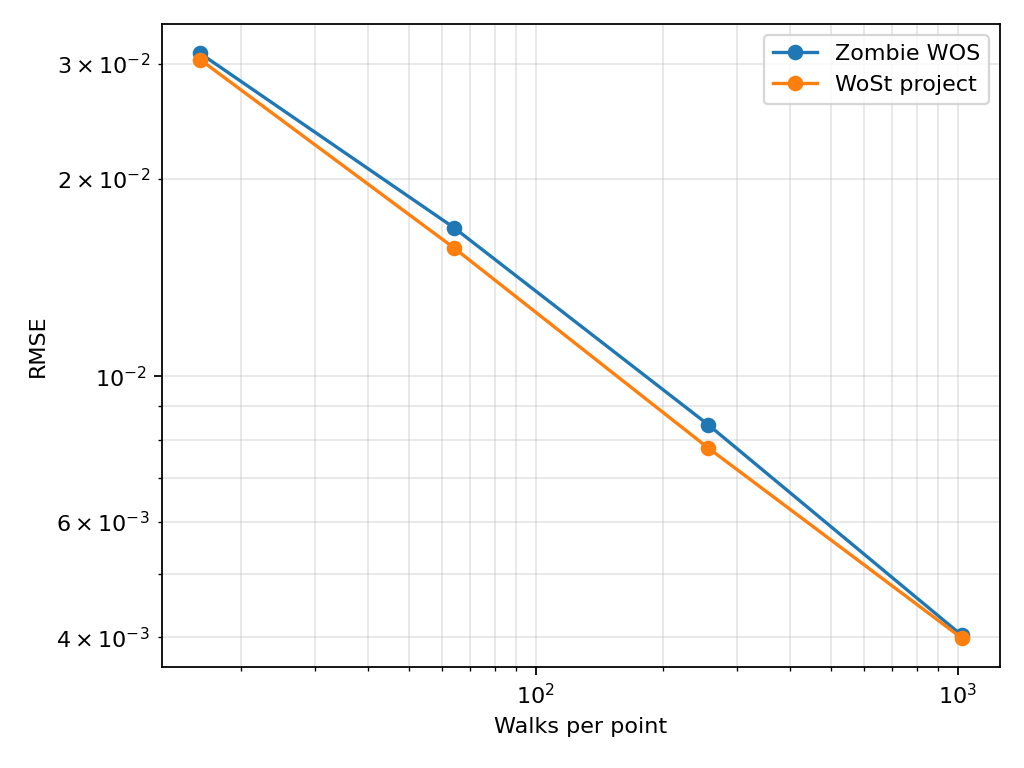
\includegraphics[width=0.72\textwidth]{experiments/final_report_figures/formal_dirichlet_rmse_vs_walks_comparison.png}
\end{center}

\textbf{Analysis.} The RMSE decreases as the number of walks increases, matching the expected Monte Carlo trend $O(N^{-1/2})$.  Zombie is faster in this Dirichlet solve-loop benchmark, but WoSt is slightly more accurate in the fresh Bunny run.

%==============================================================================
\section{2. Mixed Neumann: WoSt Uses Much Shorter Paths}
%==============================================================================

\begin{center}
\begin{tabular}{>{\bfseries}lcccc}
\toprule
Walks/query & Zombie RMSE & WoSt RMSE & Zombie steps & WoSt steps\\
\midrule
16 walks   & 0.04048 & 0.04140 & 282.19 & 30.93\\
256 walks  & 0.01726 & 0.01308 & 238.82 & 34.46\\
1024 walks & 0.01309 & 0.01141 & 239.65 & 34.47\\
\bottomrule
\end{tabular}
\end{center}

\begin{center}
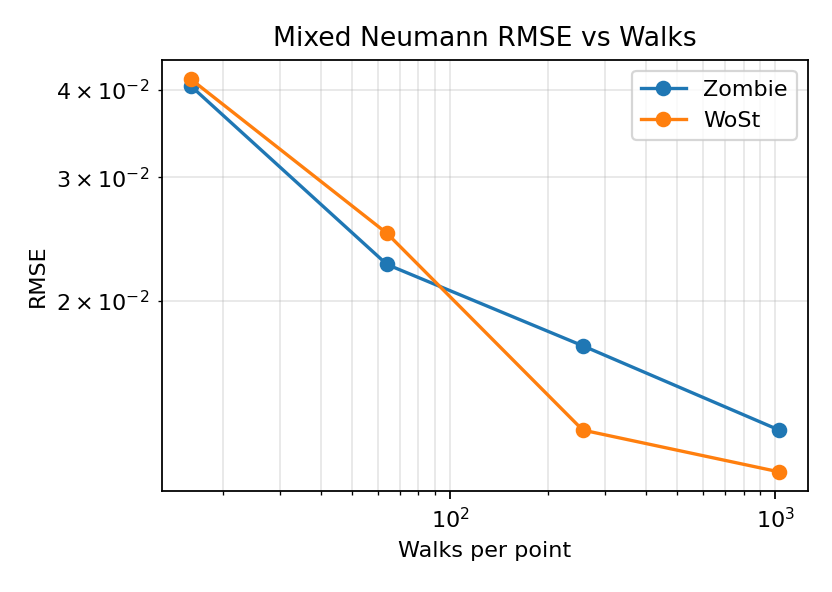
\includegraphics[width=0.72\textwidth]{experiments/final_report_figures/formal_neumann_rmse_vs_walks_comparison.png}
\end{center}

\textbf{Analysis.} Both solvers converge with more walks.  The key difference is path behavior: Zombie uses much longer reflected paths, while WoSt achieves comparable or better high-sample RMSE with far fewer mean steps.  This explains why WoSt is faster on the mixed Neumann grid.

%==============================================================================
\section{3. Boundary Bias: Epsilon Controls Neumann Reliability}
%==============================================================================

\begin{center}
\begin{tabular}{>{\bfseries}lcccc}
\toprule
Neumann $\varepsilon$ & Zombie RMSE & WoSt RMSE & Zombie steps & WoSt steps\\
\midrule
$10^{-2}$ & 0.01664 & 0.15294 & 109.81 & 6.75\\
$10^{-3}$ & 0.01280 & 0.02676 & 235.35 & 15.90\\
$10^{-4}$ & 0.01532 & 0.01249 & 251.10 & 32.21\\
$10^{-5}$ & 0.01418 & 0.01398 & 257.10 & 48.88\\
\bottomrule
\end{tabular}
\end{center}

\begin{center}
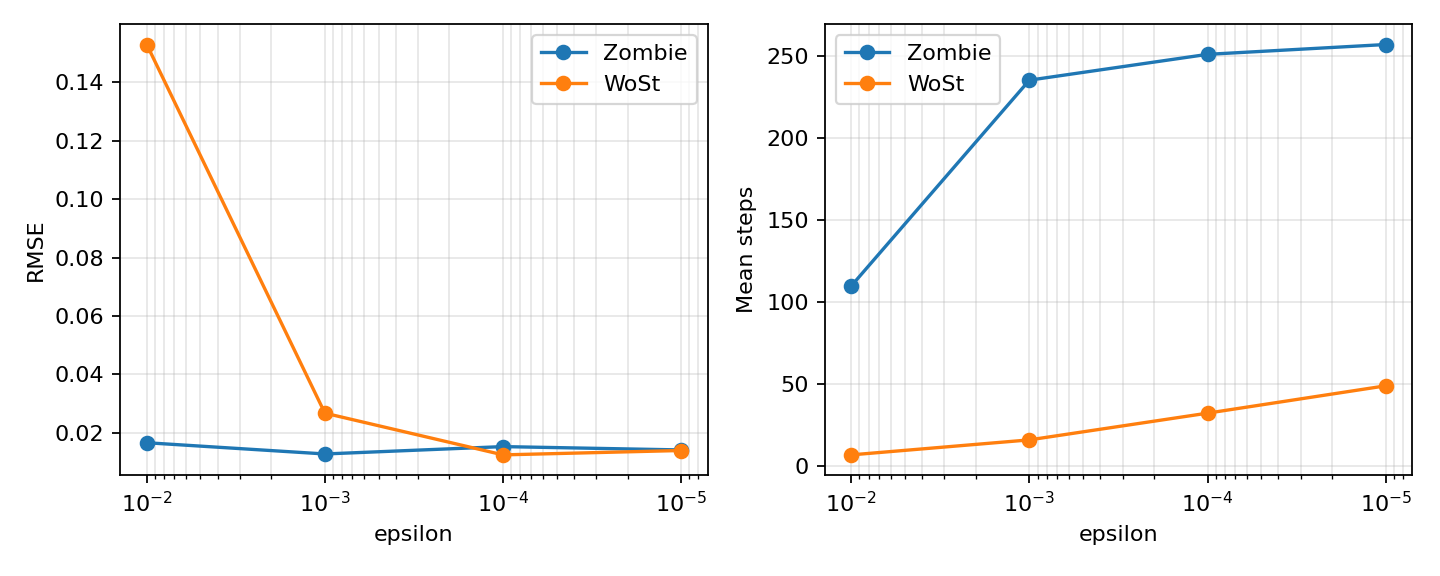
\includegraphics[width=0.72\textwidth]{experiments/final_report_figures/formal_neumann_epsilon_tradeoff_comparison.png}
\end{center}

\textbf{Analysis.} WoSt is very fast at coarse $\varepsilon$, but $\varepsilon=10^{-2}$ produces large Neumann boundary bias.  Tightening to $10^{-4}$ removes most of this bias while keeping WoSt faster than Zombie.  This directly motivates our new boundary-bias detector.

%==============================================================================
\section{4. Innovation: Self-Diagnostic WoSt}
%==============================================================================

\begin{center}
\begin{tabular}{>{\bfseries}lccc}
\toprule
Diagnostic mode & Key output & Quantitative result & Why it matters\\
\midrule
Walk Path Debugger & traced paths & 64 walks in 0.0509s & makes WoSt visually explainable\\
Bias Detector & $|u_\varepsilon-u_{\varepsilon/2}|$ grid & mean bias 0.00601 & flags epsilon-sensitive regions\\
Variance Adaptive & pilot variance allocation & samples 1024 $\to$ 562 & reduces cost with controlled RMSE\\
\bottomrule
\end{tabular}
\end{center}

\begin{center}
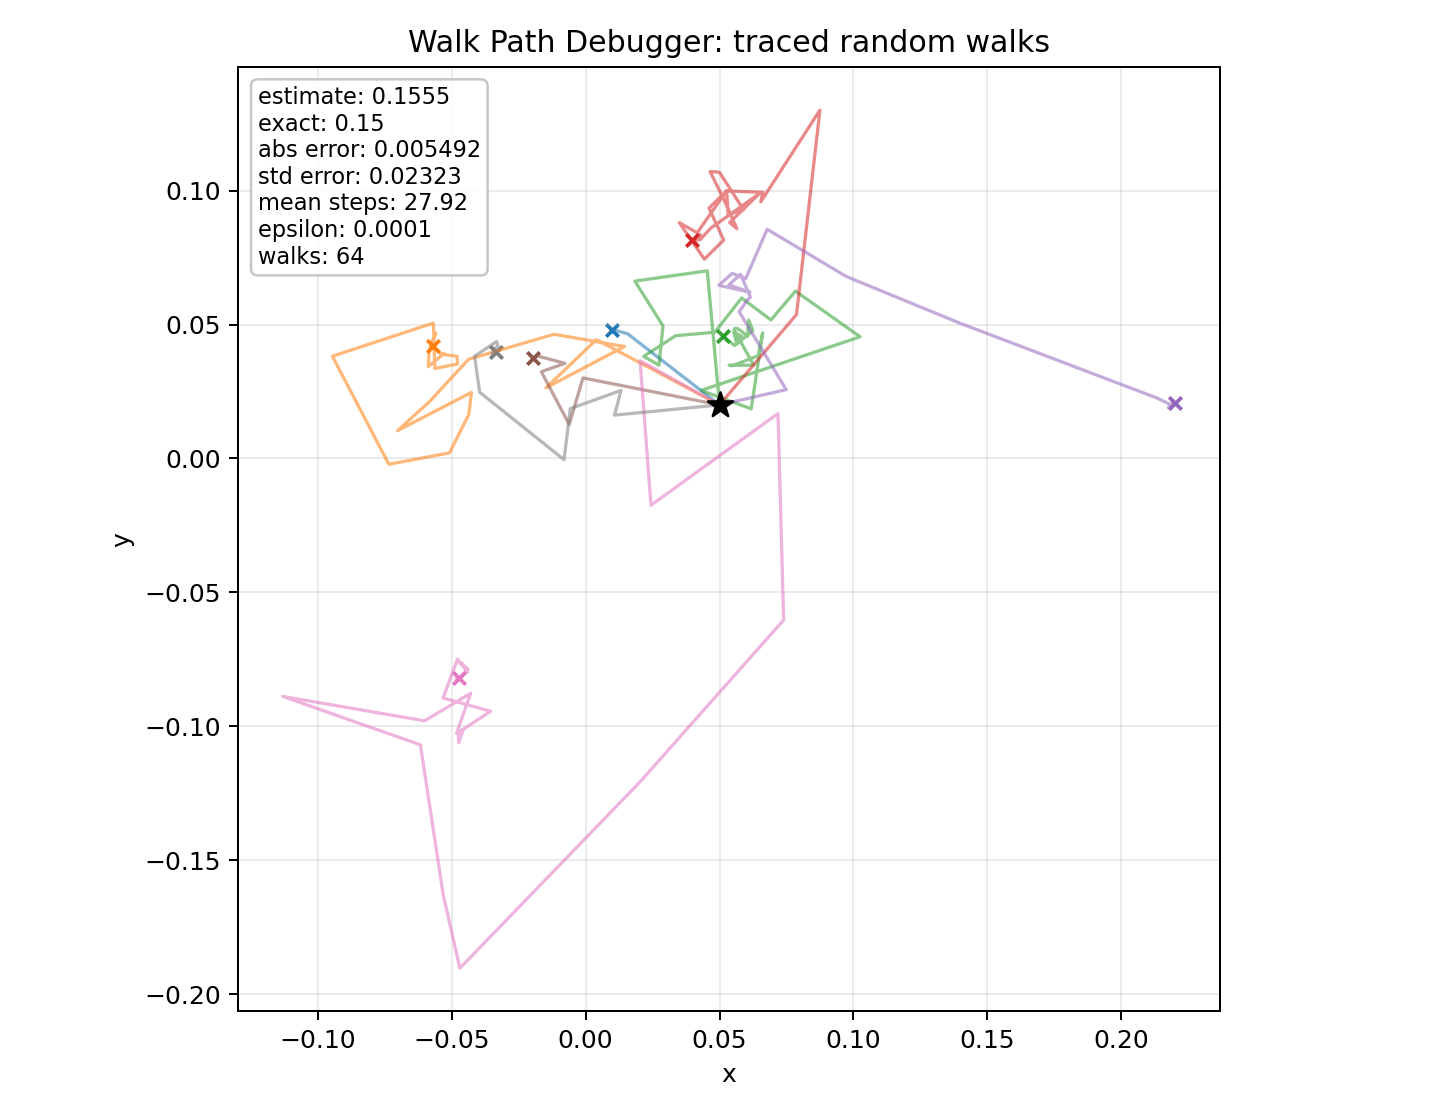
\includegraphics[width=0.47\textwidth]{experiments/final_report_figures/innovation_live_trace_plot.png}
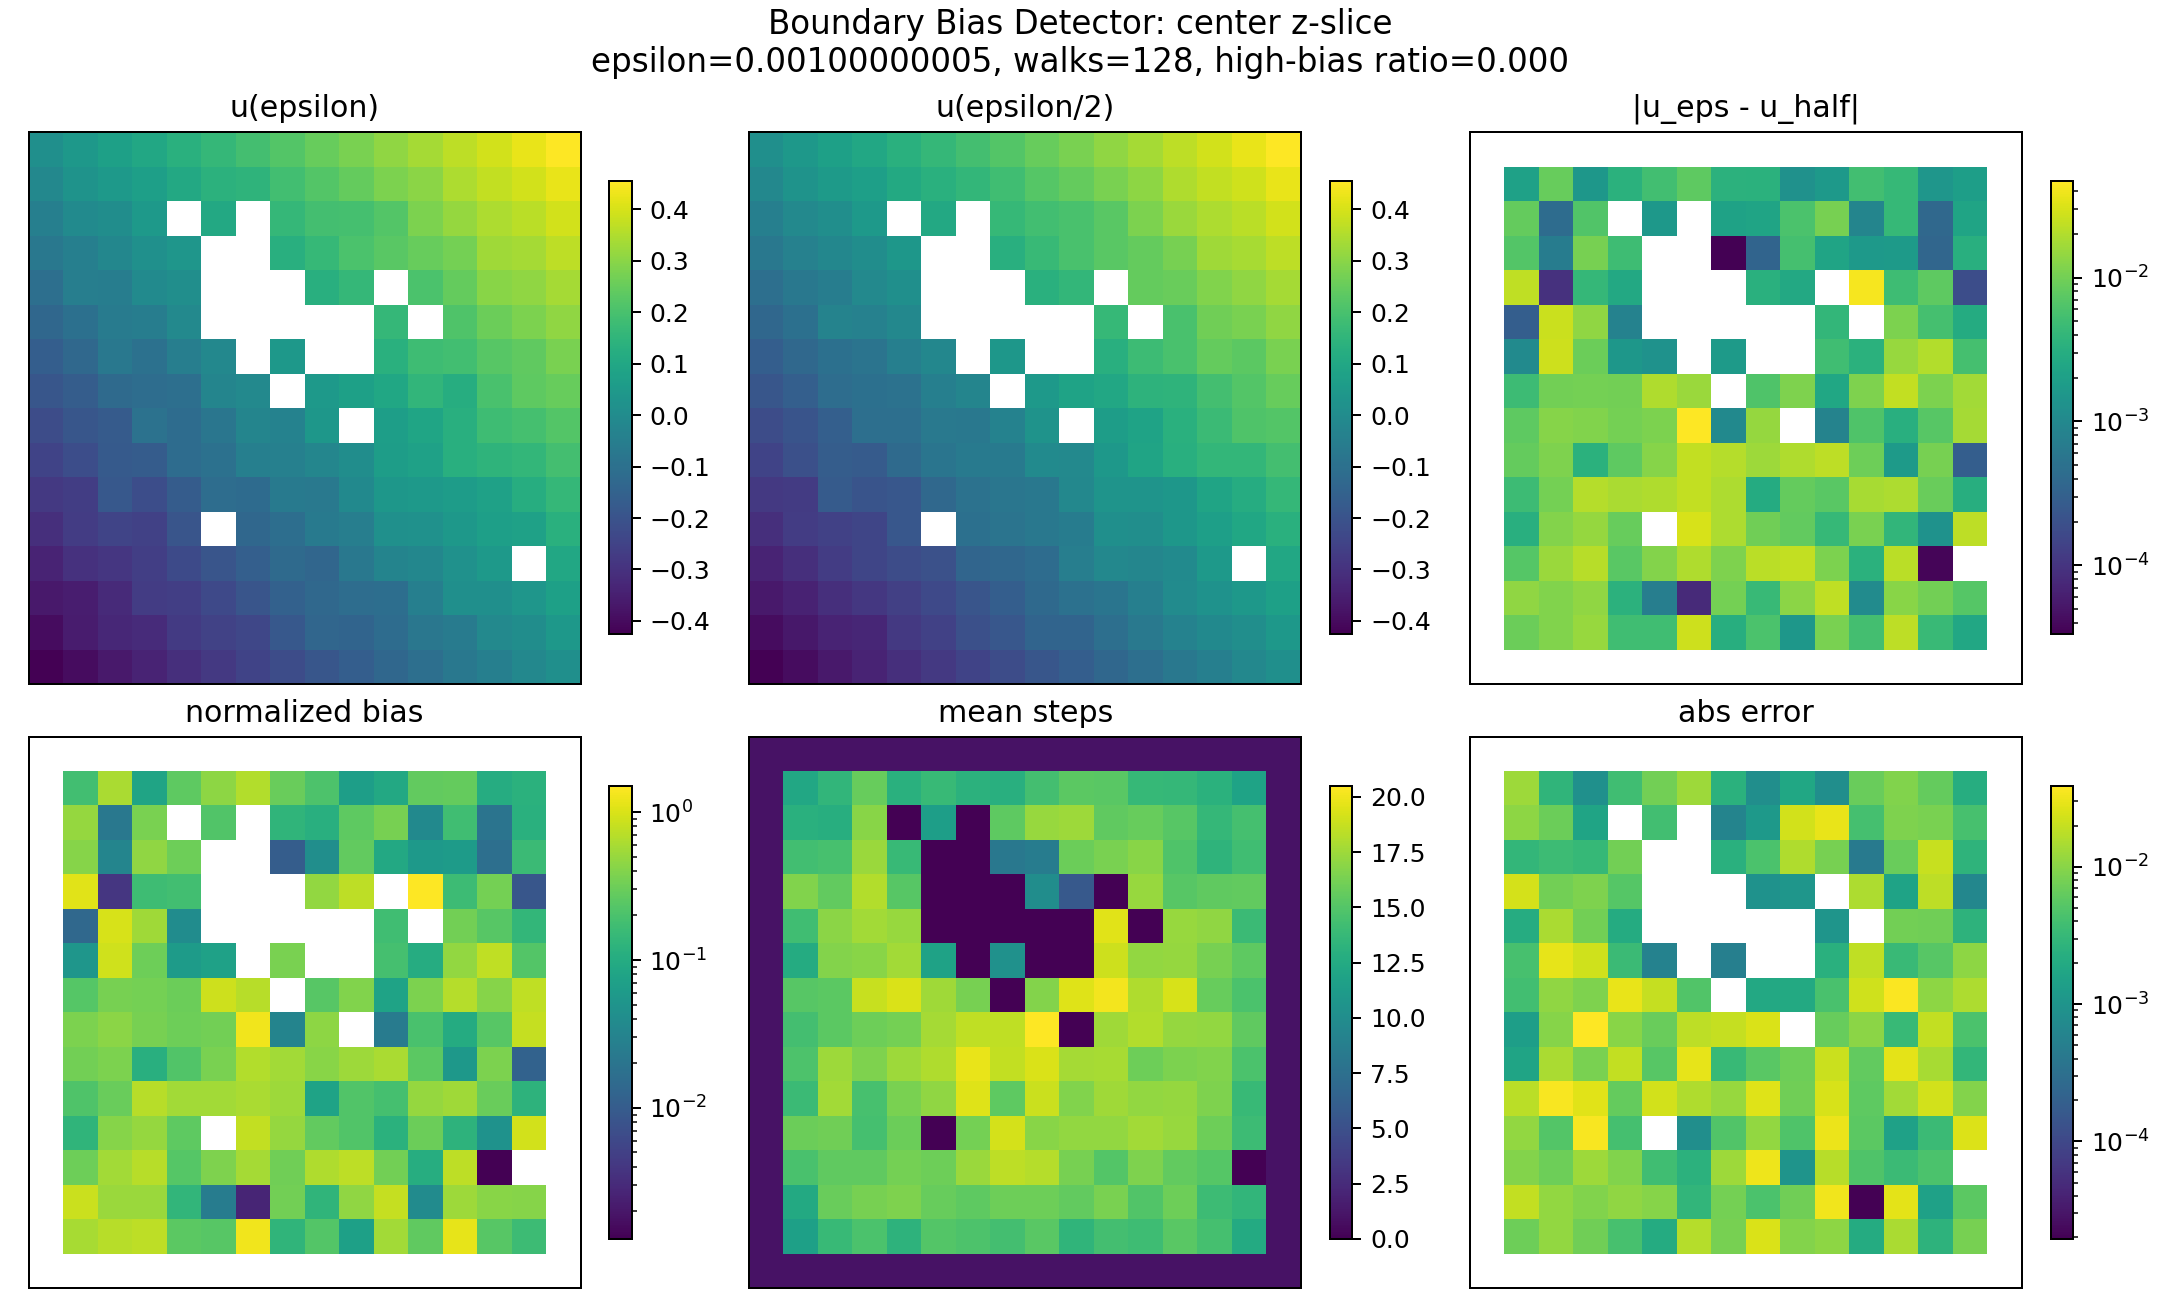
\includegraphics[width=0.47\textwidth]{experiments/final_report_figures/innovation_boundary_bias_detector.png}
\end{center}

\textbf{Analysis.} These modes turn WoSt from a black-box estimator into a solver that can explain its own behavior: where walks go, where $\varepsilon$ is unreliable, and where more samples are statistically justified.

%==============================================================================
\section{5. Variance-Predicted Adaptive Sampling Trade-off}
%==============================================================================

\begin{center}
\begin{tabular}{>{\bfseries}lccc}
\toprule
Method & RMSE & Mean samples & Runtime\\
\midrule
fixed\_512 & 0.00549 & 512.00 & 27.03s\\
fixed\_1024 & 0.00404 & 1024.00 & 53.97s\\
adaptive $\tau=0.003$ & 0.00442 & 794.80 & 45.81s\\
adaptive $\tau=0.005$ & 0.00543 & 562.48 & 33.20s\\
adaptive $\tau=0.008$ & 0.00880 & 263.78 & 16.58s\\
\bottomrule
\end{tabular}
\end{center}

\begin{center}
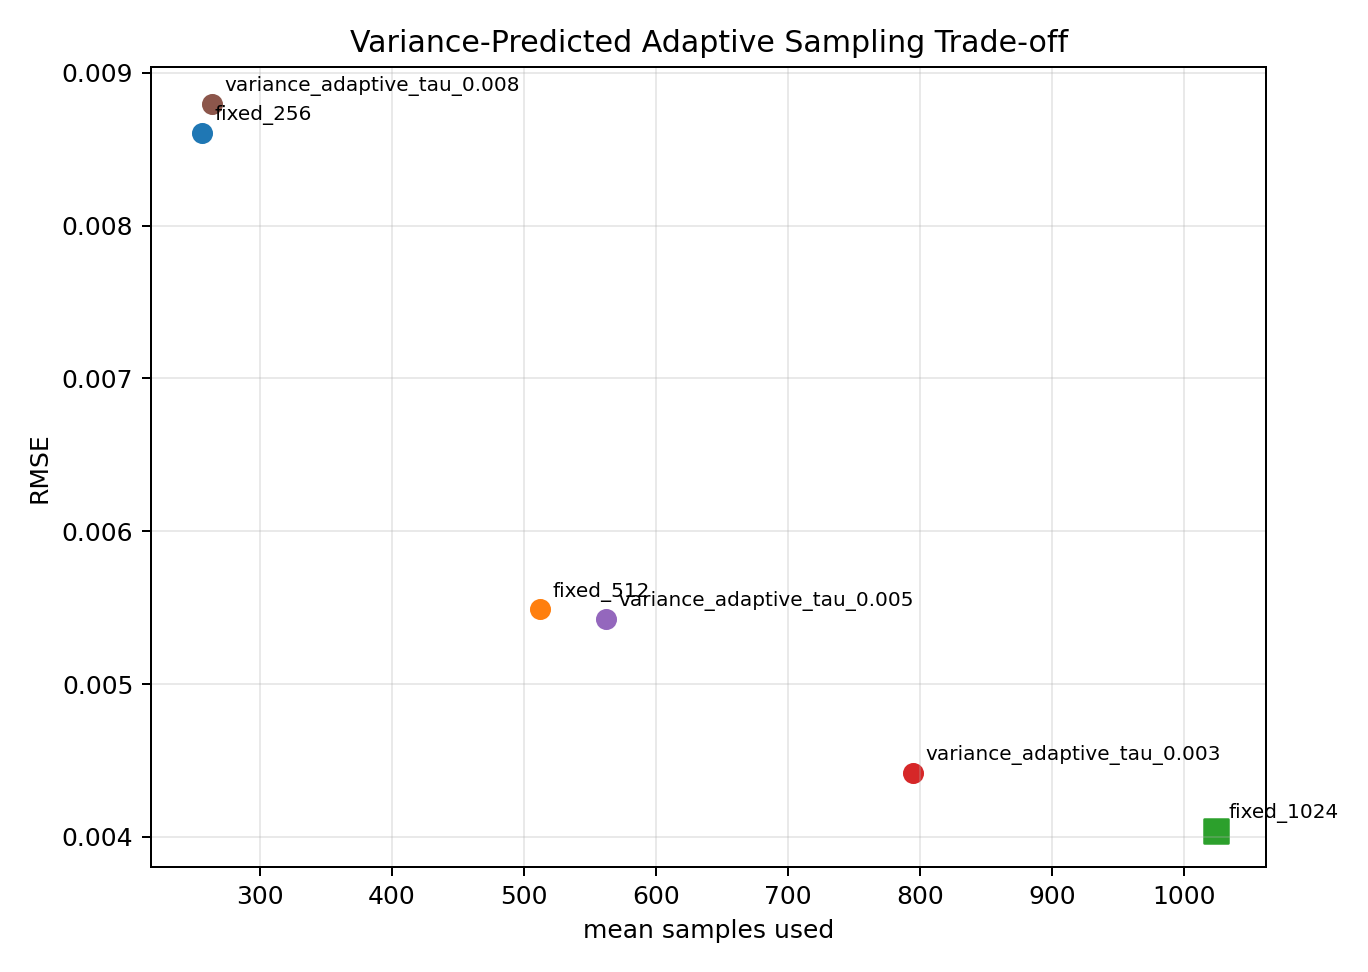
\includegraphics[width=0.47\textwidth]{experiments/final_report_figures/innovation_variance_adaptive_tradeoff.png}
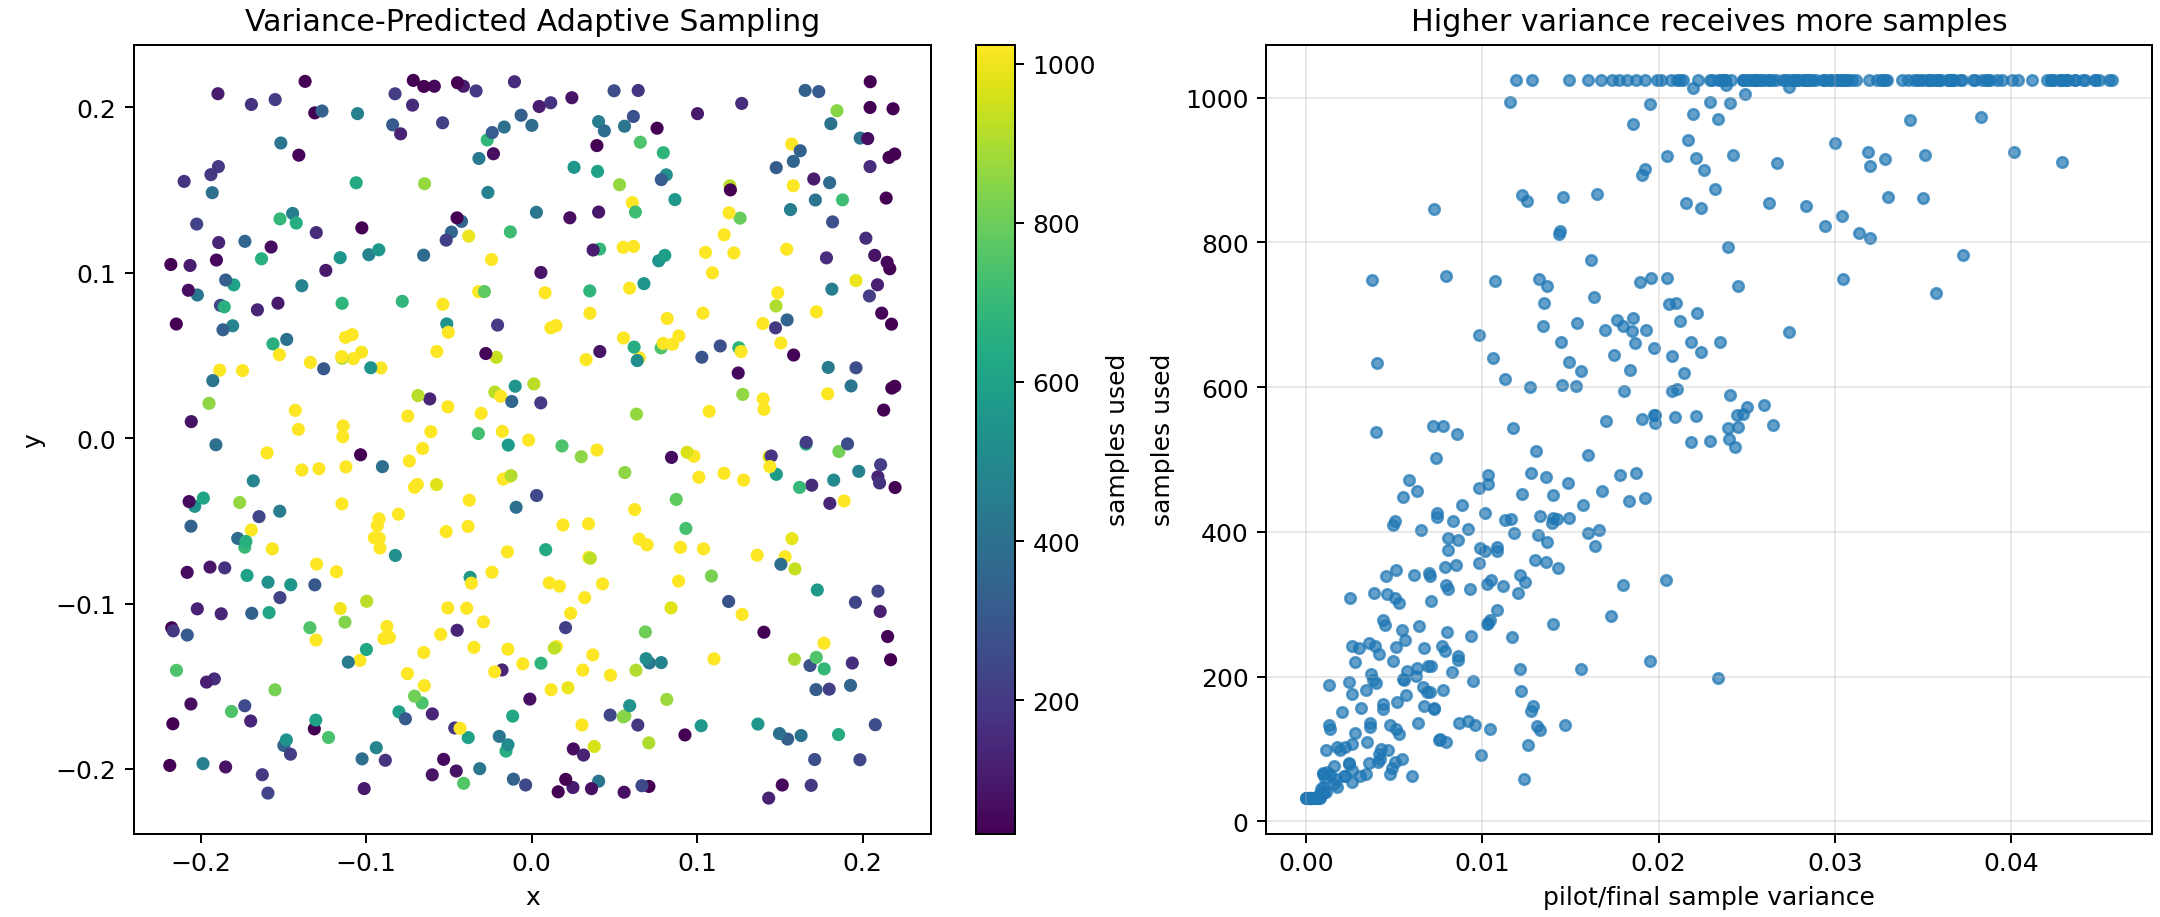
\includegraphics[width=0.47\textwidth]{experiments/final_report_figures/innovation_variance_adaptive_samples_map.png}
\end{center}

\textbf{Analysis.} The most useful live-demo setting is $\tau=0.005$: it reduces average samples by about \textbf{45.1\%} relative to fixed 1024 and reduces runtime by about \textbf{38.5\%}, while RMSE rises moderately from 0.00404 to 0.00543.  The samples map shows that high-variance regions receive more walks.

%==============================================================================
\section{Conclusions}
%==============================================================================

\begin{tcolorbox}[colback=lightbg,colframe=accent,boxrule=0.5pt,arc=2pt,left=6pt,right=6pt,top=4pt,bottom=4pt]
\textbf{What the experiments establish:}
\begin{itemize}
  \item \textbf{Correctness:} WoSt matches Zombie on the Bunny Dirichlet benchmark and follows the expected Monte Carlo convergence trend as walks increase.
  \item \textbf{Mixed-boundary behavior:} Neumann accuracy is controlled by both variance and boundary bias; coarse $\varepsilon$ is fast but can be unreliable.
  \item \textbf{Efficiency:} In mixed Neumann tests, WoSt reaches competitive accuracy with much shorter mean paths than Zombie.
  \item \textbf{Optimization-aware contribution:} walk tracing, epsilon-vs-half-epsilon bias detection, and variance-predicted sampling make the solver inspectable and tunable.
\end{itemize}
\end{tcolorbox}

\textbf{Final takeaway.} Our project goes beyond reproducing Walk-on-Stars: it turns WoSt into a \textbf{self-diagnostic and optimization-aware solver} for complex mesh domains.  The solver not only estimates the PDE solution, but also reveals where walks go, where boundary bias appears, and where additional samples are statistically worth spending.

\end{document}
